\documentclass[11pt]{article}
\usepackage[utf8]{inputenc}
\usepackage{amsmath}
\usepackage{amssymb}
\usepackage{amsthm}
\usepackage{tcolorbox}
\usepackage{tikz}
\usetikzlibrary{positioning}
\usepackage{graphicx}


\newcommand{\argmax}[1]{\underset{#1}{\operatorname{arg}\,\operatorname{max}}\;}
\newcommand{\expectation}[1]{\mathbb{E}\left[#1\right]}
\newcommand{\x}{{\bf x}}
\newcommand{\z}{{\bf z}}

\newtheorem{proposition}{Proposition}[section]

\title{Kalman Filters: an introduction}
\author{Gerardo Durán Martín}
\begin{document}
\maketitle

\section{Introduction}

Dynamical systems are models that capture the time evolution of a system. A discrete-time linear dynamical system is a dynamical system in which an $M$-dimensional vector ${\bf x}_n$ evolves in the form.

\begin{equation}
	{\bf x}_{n+1} = {\bf A x}_n
\end{equation}

% An example of a linear dynamical system is...
\begin{figure}[h!]
	\centering
	\includegraphics[scale=0.5]{../figures/discrete-dynamical-system}
	\caption{Example of a discrete-time dynamical system.}
	\label{fig:discrete-dynamical-system}
\end{figure}



In this work, are interested in dynamical systems that depend on some unobserved signal, usually called latent variables, and a set of observed values that are directly derived from the source signal. We define the set of observed variables ${\bf X}=\left\{{\bf x}_n \vert {\bf x}_n \in \mathbb{R}^M\right\}$ as the observed dataset, and the set of latent variables ${\bf Z}=\left\{{\bf z}_n \vert {\bf z}_n \in \mathbb{R}^K\right\}$ as the latent dataset. We also denote $\mathcal{D} = ({\bf X}, {\bf Z})$ as the complete-data set.

One way to represent such system is to assume the existence of an unobserved signal ${\bf z}_n$ that evolves over time according to the matrix ${\bf A}\in\mathbb{R}^{K\times K}$. Once ${\bf z}_{n}$ is updated, the observed value ${\bf x}_{n+1}$ is the result of a linear transformation for ${\bf z}_{n+1}$ induced by the matrix ${\bf C}\in \mathbb{R}^{M\times K}$. The equations that govern such system can be written in the form:

\begin{align*}
	{\bf z}_{n+1} &= {\bf A} {\bf z}_{n}\\
	{\bf x}_{n+1} &= {\bf C} {\bf z}_{n+1}
\end{align*}

An example of such system is presented in Figure \ref{fig:hidden-dynamical-system}, in which the dynamics of the vector ${\bf x}_n$ is completely determined by the vector ${\bf z}_n$. Hence, the evolution of the system is completely determined by the initial condition ${\bf z}_0$. Assuming that ${\bf z}_0$ is known and we observed a fixed number of observations ${\bf X}$, the problem reduces to find matrices ${\bf A}$ and ${\bf C}$ that generated the observed values.

% An example of a linear dynamical system is...
\begin{figure}[h!]
	\centering
	\includegraphics[scale=0.5]{../figures/hidden-dynamical-system}
	\caption{Example of a hidden dynamical system.}
	\label{fig:hidden-dynamical-system}
\end{figure}

In some settings, however, we assume that the underlying signal ${\bf z}_n$ and the observed value ${\bf x}_n$ does not behave deterministically. To consider an example, suppose we are interested in modelling the behaviour of a stock. We assume that the stock has an underlying signal that is then affected by stochastic market forces and corrupts its underlying value. Under this scenario, ${\bf X}$ is a dataset of sampled random values that were generated by some unseen dataset ${\bf Z}$. Our goal in this work is to find a probabilistic model that efficiently estimates the parameters of our model, and a procedure to determine the plausible dataset $\bf Z$. 

% as we will see, the procedure can be achieved by the EM-algorithm and the dataset Z can be found using a known algorithm known as the Kalman-filter equations.

\subsection{Stochastic Linear Dynamical Systems}
We begin this section by modifying our previous system to take into account the uncertainty in the system. As previously mentioned, we assume that that both the underlying signal and the observed signal are corrupted by some noise.
 

\begin{align*}
	{\bf z}_{n+1} &= {\bf A} {\bf z}_{n} + \boldsymbol\varepsilon_n\\
	{\bf x}_{n+1} &= {\bf C} {\bf z}_{n+1} + \boldsymbol\varphi_n
\end{align*}

The noise terms $\boldsymbol{\varepsilon}_n$, and $\boldsymbol{\varphi}_n$ are assumed to be normally distributed with mean zero and covariance matrices $\boldsymbol{\Gamma}$, and $\boldsymbol{\Sigma}$.

Given the structure of the dynamical system, the likelihood of the model is given by

\begin{equation}
	p({\bf X}, {\bf Z}\vert\boldsymbol\theta) = p({\bf z}_1)\prod_{n=2}^N p({\bf z}_n\vert {\bf z}_{n-1})\prod_{n=1}^N p({\bf x}_n\vert {\bf z}_n)
\end{equation}

% to-do: Add equations for the initial condition z0
We can also represent this system as a graphical model as specified in Figure \ref{fig:lds-gm}.

\begin{figure}
	\centering
	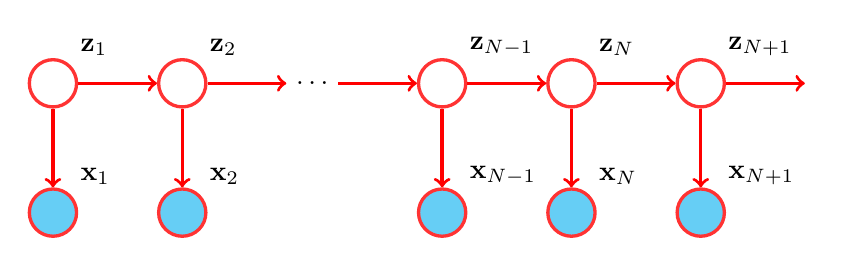
\begin{tikzpicture}[
latentnode/.style={circle, draw=red!80, minimum size=6mm, very thick},
observednode/.style={circle, draw=red!80, fill=cyan!60, minimum size=6mm, very thick},
]

% Defining the nodes
\node[latentnode, label=above right:{${\bf z}_1$}] (z1) {};
\node[latentnode, label=above right:{${\bf z}_2$}] (z2) [right=of z1] {};
\node (transition) [right=of z2] {$\ldots$};
\node[latentnode, label=above right:{${\bf z}_{N-1}$}] (z_nm1) [right=of transition] {};
\node[latentnode, label=above right:{${\bf z}_{N}$}] (zn) [right=of z_nm1] {};
\node[latentnode, label=above right:{${\bf z}_{N+1}$}] (z_np1) [right=of zn] {};
\node (final) [right=of z_np1] {};

% Defining observed nodes
\node[observednode, label=above right:{${\bf x}_1$}] (x1) [below=of z1]{};
\node[observednode, label=above right:{${\bf x}_2$}] (x2) [below=of z2]{};
\node[observednode, label=above right:{${\bf x}_{N-1}$}] (x_nm1) [below=of z_nm1]{};
\node[observednode, label=above right:{${\bf x}_{N}$}] (xn) [below=of zn]{};
\node[observednode, label=above right:{${\bf x}_{N+1}$}] (x_np1) [below=of z_np1]{};


% Relationships between latent variables
\draw[->, color=red, very thick] (z1) -- (z2);
\draw[->, color=red, very thick] (z2) -- (transition);
\draw[->, color=red, very thick] (transition) -- (z_nm1);
\draw[->, color=red, very thick] (z_nm1) -- (zn);
\draw[->, color=red, very thick] (zn) -- (z_np1);
% final node
\draw[->, color=red, very thick] (z_np1) -- (final);

% Relationships between observed and latent variables
\draw[->, color=red, very thick] (z1) -- (x1);
\draw[->, color=red, very thick] (z2) -- (x2);
\draw[->, color=red, very thick] (z_nm1) -- (x_nm1);
\draw[->, color=red, very thick] (zn) -- (xn);
\draw[->, color=red, very thick] (z_np1) -- (x_np1);

\end{tikzpicture}
	\caption{Graphical representation of a linear dynamical system with latent variables. The filled circles represent observed datapoints, whereas the empty circles represent latent variables.}
	\label{fig:lds-gm}
\end{figure}


Our purpose is to find parameters $\boldsymbol\theta = \{{\bf A}, {\bf C}, \boldsymbol\Gamma, \boldsymbol\Sigma, \boldsymbol\mu_0, {\bf V}_0\}$ that best represent the data. This is usually done maximising the likelihood of the data with respect to the parameters $\boldsymbol{\theta}$. Maximising the likelihood of this model, however, is not straightforward. This is because the only observed data we have is given by the dataset $\bf X$. % Explain more this step


One approach of finding such parameters is to make use of the EM algorithm: an iterative approach to maximise the likelihood of the complete-data log-likelihood as follows

\begin{align}
	\boldsymbol{\theta}^\text{new} &= \argmax{\boldsymbol{\theta}} \mathbb{E}_{{\bf Z}\vert {\bf X}, \boldsymbol{\theta}^\text{old}}[\log p({\bf X}, {\bf Z}\vert \boldsymbol\theta)]\\
	&= \argmax{\boldsymbol{\theta}} Q(\boldsymbol\theta, \boldsymbol\theta^\text{old})
\end{align}

Where we have defined $Q(\boldsymbol\theta, \boldsymbol\theta^\text{old}) := \mathbb{E}_{{\bf Z}\vert {\bf X}, \boldsymbol{\theta}^\text{old}}[\log p({\bf X}, {\bf Z}\vert \boldsymbol\theta)]$.The computation of the posterior probability of latent variables $p({\bf Z}\vert {\bf X}, \boldsymbol\theta)$ is called the E-step. The maximisation of the complete-data log-likelihood with respect to the posterior latent variables is called the M-step.


\subsection{The E-step}
To make use of the E-step, it is helpful to distinguish which elements depend on ${\bf z}_n$. Consider

\begin{align}
	\log p({\bf X}, {\bf Z}\vert \boldsymbol\theta) &= \log p({\bf z}_1) + \sum_{n=2}^N \log p({\bf z}_n\vert {\bf z}_{n-1}) + \sum_{n=1}^N \log p({\bf x}_n\vert {\bf z}_n)\\
	   &=\frac{1}{2}\log\vert{\bf V}_0^{-1}\vert - \frac{1}{2}({\bf z}_1 - \boldsymbol\mu_0)^T{\bf V}_0^{-1}({\bf z}_1 - \boldsymbol\mu_0) \nonumber \\
	   &\hspace{1cm}+ \sum_{n=2}^N \frac{1}{2}\log\vert\boldsymbol\Gamma^{-1}\vert - \frac{1}{2}({\bf z}_n - {\bf A z}_{n-1})^T\boldsymbol{\Gamma}^{-1}({\bf z}_n - {\bf A z}_{n-1}) \nonumber \\
	   &\hspace{1cm}+\sum_{n=1}^N \frac{1}{2}\log\vert\boldsymbol\Sigma\vert -\frac{1}{2}({\bf x}_n - {\bf C z}_n)^T \boldsymbol{\Sigma}^{-1}({\bf x}_n - {\bf C z}_n) + \text{const.}\\
	   &= \frac{1}{2}\log \vert
	  {\bf V}_0^{-1}\vert -\frac{1}{2}\left[\text{Tr}\left({\bf z}_1 {\bf z}_1^T {\bf V}_0^{-1}\right) -2 {\bf z}_1^T{\bf V}_0^{-1}\boldsymbol\mu_0 + \boldsymbol\mu_0^T {\bf V}_0^{-1}\boldsymbol\mu_0\right] \nonumber \\
	  &\hspace{1cm}+ \frac{N-1}{2}\log\vert\boldsymbol\Gamma^{-1}\vert + \frac{N}{2}\log\vert \boldsymbol\Sigma^{-1}\vert \nonumber \\
	  &\hspace{1cm}-\frac{1}{2} \sum_{n=2}^{N}\text{Tr}\left({\bf z}_n{\bf z}_n^T\boldsymbol\Gamma^{-1} -2 {\bf z}_{n-1}{\bf z}_n^T{\bf A}\boldsymbol\Gamma^{-1} +  {\bf z}_{n-1}{\bf z}_{n-1}^T{\bf A}\boldsymbol\Gamma^{-1}{\bf A}\right) \nonumber\\
	  &\hspace{1cm}-\frac{1}{2}\sum_{n=1}^N\left[{\bf x}_n^T\boldsymbol{\Sigma}^{-1}{\bf x}_n-2{\bf z}_n^T\boldsymbol\Sigma^{-1}{\bf x}_n + \text{Tr}({\bf z}_n{\bf z}_n^T{\bf C}\boldsymbol\Sigma^{-1}{\bf C})\right] \nonumber\\
	  &\hspace{1cm} + \text{const.}
\end{align}

Where const. are the terms that do not depend on $\boldsymbol{\theta}$. From this last equation, we note that the expectation with respect to the posterior distribution comes only in the form of the expectations $\mathbb{E}[{\bf z}_n]$, $\mathbb{E}[{\bf z}_n{\bf z}_{n}^{T}]$, and  $\mathbb{E}[{\bf z}_n{\bf z}_{n-1}^{T}]$. We obtain:

\begin{align}
	Q(\boldsymbol\theta, \boldsymbol\theta^\text{old}) &= \frac{1}{2}\log \vert
	  {\bf V}_0^{-1}\vert -\frac{1}{2}\left[\text{Tr}\left(\mathbb{E}\left[{\bf z}_1 {\bf z}_1^T\right] {\bf V}_0^{-1}\right) -2 \mathbb{E}\left[{\bf z}_1\right]^T{\bf V}_0^{-1}\boldsymbol\mu_0 + \boldsymbol\mu_0^T {\bf V}_0^{-1}\boldsymbol\mu_0\right] \nonumber \\
	  &\hspace{1cm}+ \frac{N-1}{2}\log\vert\boldsymbol\Gamma^{-1}\vert + \frac{N}{2}\log\vert \boldsymbol\Sigma^{-1}\vert \nonumber \\
	  &\hspace{1cm}-\frac{1}{2} \sum_{n=2}^{N}\text{Tr}\left(\mathbb{E}\left[{\bf z}_n{\bf z}_n^T\right]\boldsymbol\Gamma^{-1} -2\mathbb{E}\left[ {\bf z}_{n-1}{\bf z}_n^T\right]{\bf A}\boldsymbol\Gamma^{-1} + \mathbb{E}\left[{\bf z}_{n-1}{\bf z}_{n-1}^T\right]{\bf A}\boldsymbol\Gamma^{-1}{\bf A}\right) \nonumber\\
	  &\hspace{1cm}-\frac{1}{2}\sum_{n=1}^N\left[{\bf x}_n^T\boldsymbol{\Sigma}^{-1}{\bf x}_n-2\mathbb{E}\left[{\bf z}_n^T\right]\boldsymbol\Sigma^{-1}{\bf x}_n + \text{Tr}(\mathbb{E}\left[{\bf z}_n{\bf z}_n^T\right]{\bf C}\boldsymbol\Sigma^{-1}{\bf C})\right] \nonumber\\
	  &\hspace{1cm} + \text{const.} \label{eq:Q-LDS}
\end{align}

Before computing the expected values of the latent variables, it is useful to find the posterior distributions of the latent variables $\gamma({\bf z}_n) := p({\bf z}_n\vert {\bf X})$, and $\xi({\bf z}_{n-1}, {\bf z}_{n}) := p({\bf z}_{n-1}, {\bf z}_n\vert {\bf X})$. %why is it useful?

\begin{proposition}
	The term $\gamma({\bf z}_n)$ can be written as a product of the joint probabilities of the first $n$ observations and ${\bf z}_n$, and the conditional probability of the observations that follow ${\bf z}_n$ conditional on ${\bf z}_n$.
\end{proposition}

\begin{proof}\label{prop:gamma-factorisation}
Consider  $\gamma({\bf z}_n)$ and equation \ref{gm:1} from proposition \ref{prop:graphical-models-separation}. We have
\begin{align}
	\gamma({\bf z}_n) &= p({\bf z}_n \vert {\bf X})\\
					  &= \frac{1}{p({\bf X})}p({\bf z}_n)p({\bf X} \vert {\bf z}_n)\\
					  &= \frac{1}{p({\bf X})} p({\bf z}_n) p({\bf x}_1, \ldots, {\bf x}_n\vert {\bf z}_n) p({\bf x}_{n+1}, \ldots, {\bf x}_N\vert {\bf z}_n)\\
					  &= \frac{1}{p({\bf X})}p({\bf x}_1, \ldots, {\bf x}_n, {\bf z}_n) p({\bf x}_{n+1}, \ldots, {\bf x}_N\vert {\bf z}_n)\\
					  &= \frac{1}{p({\bf X})}\alpha({\bf z}_n)\beta({\bf z}_n)
\end{align}

Where we have defined $\alpha({\bf z}_n) := p({\bf x}_1, \ldots, {\bf x}_n, {\bf z}_n)$ as the joint probability of the observed data up to $n$, and $\beta({\bf z}_n) := p({\bf x}_{n+1}, \ldots, {\bf x}_N\vert {\bf z}_n)$ as the probability of all data that follows the $n$-th observation, conditional on the $n$-th latent variable ${\bf z}_n$.
\end{proof}


% Here we show that the xi can also be written in terms of alpha and beta
\begin{proposition}\label{prop:xi-factorisation}
	The term $\xi({\bf z}_{n-1}, {\bf z}_n)$ can be written in terms of $\alpha({\cdot})$, and $\beta(\cdot)$
\end{proposition}

\begin{proof}
	\begin{align}
		\xi({\bf z}_{n-1}, {\bf z}_{n}) &= p({\bf z}_{n-1}, {\bf z}_{n} \vert {\bf X})\\
		&= \frac{1}{p({\bf X})}p({\bf z}_{n-1}, {\bf z}_{n}) p({\bf X} \vert {\bf z}_{n-1}, {\bf z}_{n})\\
		&= \frac{1}{p({\bf X})} p({\bf z}_{n-1}) p({\bf z}_{n} \vert {\bf z}_{n-1}) p({\bf x}_1, \ldots, {\bf x}_{n-1}\vert {\bf z}_{n-1}) \nonumber \\
			&\hspace{1cm} p({\bf x}_n\vert {\bf z}_n) p({\bf x}_{n+1}, \ldots, {\bf x}_N \vert {\bf z}_n)\\
		&= \frac{1}{p({\bf X})} p({\bf z}_{n} \vert {\bf z}_{n-1}) p({\bf x}_1, \ldots, {\bf x}_{n-1}, {\bf z}_{n-1}) \nonumber \\
			&\hspace{1cm} p({\bf x}_n\vert {\bf z}_n) p({\bf x}_{n+1}, \ldots, {\bf x}_N \vert {\bf z}_n)\\
		&= \frac{1}{p({\bf X})} \alpha({\bf z}_{n-1}) p({\bf z}_{n} \vert {\bf z}_{n-1}) p({\bf x}_n \vert {\bf z}_n) \beta({\bf z}_n)
	\end{align}
\end{proof}


% Hence, to make sense of gamma and xi we only need to find values of alpha and beta
Propositions \ref{prop:gamma-factorisation}, and \ref{prop:xi-factorisation} show that both $\gamma$ and $\xi$ are completely determined by the values of $\alpha$, and $\beta$. Hence, we only need to compute the set of values $\{\alpha({\bf z}_n)\}_n$ and $\{\beta({\bf z}_n)\}_n$ once per E-iteration to find the distributions of $\gamma$ and $\xi$. Our next step is to derive an algorithm to efficiently compute $\alpha({\bf z}_n)$, and $\beta({\bf z}_n)$ for every $n$.

% 	* We show that alpha can be represented as a recursive formula
\begin{proposition}
	$\alpha({\bf z}_n)$ can be written recursively as
	\begin{equation}
		\alpha({\bf z}_n) = p({\bf x}_n\vert {\bf z}_n) \int_{{\bf z}_{n-1}} \alpha({\bf z}_{n-1})p({\bf z}_n\vert{\bf z}_{n-1}) d{\bf z}_{n-1}
	\end{equation}
\end{proposition}

\begin{proof}
	\texttt{to-do: write proof}
\end{proof}

%  	* We show that beta can be represented as a recursive formula
\begin{proposition}
	$\beta({\bf z}_n)$ can be written recursively as
	\begin{equation}
		\beta({\bf z}_n) = \int_{{\bf z}_{n+1}} \beta({\bf z}_{n+1})p({\bf x}_{n+1}\vert {\bf z}_{n+1}) p({\bf z}_{n+1}\vert {\bf z}_n) d{\bf z}_{n+1}
	\end{equation} 
\end{proposition}

\begin{proof}
	\texttt{to-do: write proof}
\end{proof}

% We argue that alpha and beta values can become small very quick, so we require another way to compute its values
For moderately large $N$, $\alpha$ and $\beta$ become small very quick. To solve this we work with re-scaled values for $\alpha$ and $\beta$. This has the additional benefit that the re-scaled values $\alpha({\bf z}_n)$ can be written in form of a Normal distribution whose updating equations are  called the \textbf{Kalman equations}.

% Introduce alpha hat and beta hat: show that they can be written

\begin{proposition}
	Defining the scaled value $\hat\alpha({\bf z}_n)$ as
	\begin{equation}
		\hat\alpha({\bf z}_n) := \frac{\alpha({\bf z}_n)}{p({\bf x}_1, \ldots, {\bf x}_n)} = p({\bf z}_n \vert {\bf x}_1, \ldots, {\bf x}_n)
	\end{equation}
	
	results in an updating equation of the form
	
	\begin{equation}
		 c_n \hat\alpha({\bf z}_n) = p({\bf x}_n\vert{\bf z}_n)\int \hat\alpha({\bf z}_{n-1})p({\bf z}_n \vert {\bf z}_{n-1}) d{\bf z}_{n-1}
	\end{equation}
	
	with
	
	\begin{equation}
		c_n = \int_{{\bf z}_n} p({\bf x}_n \vert {\bf z}_n) \int_{{\bf z}_{n-1}} \hat\alpha({\bf z}_{n-1})p({\bf z}_n \vert {\bf z}_{n-1}) d{\bf z}_n{\bf z}_{n-1}
	\end{equation}
\end{proposition}

\begin{proof}
	\texttt{to-do: write proof}
\end{proof}

\begin{proposition}
	Defining the scaled value $\hat\beta({\bf z}_n)$ as
	\begin{equation}
		\hat\beta({\bf z}_n) = \frac{p({\bf x}_{n+1}, \ldots, {\bf x}_N \vert {\bf z}_n)}{p({\bf x}_{n+1}, \ldots, {\bf x}_N \vert {\bf x}_1, \ldots {\bf x}_n)}
	\end{equation}
	results in an updating equation of the form
	\begin{equation}
		\hat\beta({\bf z}_n) = \frac{1}{c_{n+1}}\int p({\bf x}_{n+1}\vert{\bf z}_{n+1})p({\bf z}_{n+1}\vert{\bf z}_n) d{\bf z}_{n+1}
	\end{equation}
\end{proposition}

\begin{proof}
	\texttt{to-do: write proof}
\end{proof}

The term $\hat\alpha({\bf z}_n)$ is called the $\alpha$-forward message passing for a linear dynamical system or \textbf{Kalman filter equation}.  The term $\hat\beta({\bf z}_n)$ is called the $\beta$-backward message passing of a linear dynamical system or \textbf{Kalman smoother equation}. Intuitively, $\hat\alpha({\bf z}_n)$ represents the information that the history of the data has on the $n$-th observation, whereas $\hat\beta({\bf z}_n)$ represents how a latent variable with with known value at time $n$ affects the future behaviour of the system.

In the following two propositions we show that $\gamma({\bf z}_n)$ and $\xi({\bf z}_{n-1}, {\bf z}_{n})$ can be written in terms of $\hat\alpha$ and $\hat\beta$. We later show that this induces a normal probability density function for $\gamma({\bf z}_n)$ in terms of a recursive formula that allows to efficiently compute the expected values $\mathbb{E}[{\bf z}_n]$, $\mathbb{E}[{\bf z}_n{\bf z}_{n}^{T}]$, and  $\mathbb{E}[{\bf z}_n{\bf z}_{n-1}^{T}]$.

% Show that gamma and xi can be written in terms of \hat\alpha and \hat\beta.

\begin{proposition}
	$\gamma({\bf z}_n)$ can be written in terms of the re-scaled factors $\hat\alpha({\bf z}_n)$, and $\hat\beta({\bf z}_n)$ as
	\begin{equation}
		\gamma({\bf z}_n) = \hat\alpha({\bf z}_n)\hat\beta({\bf z}_n).
	\end{equation}
\end{proposition}

\begin{proof}
	\texttt{to-do: write proof}
\end{proof}

\begin{proposition}
	$\xi({\bf z}_{n-1}, {\bf z}_n)$ can be written in terms of the re-scaled factors $\hat\alpha({\bf z}_n)$, and $\hat\beta({\bf z}_n)$ as
	\begin{equation}
		\xi({\bf z}_{n-1}, {\bf z}_{n}) = c_n^{-1}\hat\alpha({\bf z}_n)p({\bf x}_n \vert {\bf z}_n) p({\bf z}_{n-1}\vert {\bf z}_n)\hat\beta({\bf z}_n)
	\end{equation}
\end{proposition}

\begin{proof}
	\texttt{to-do: write proof}
\end{proof}


As we have previously noted, the term $\hat\alpha({\bf z}_n)$ can be represented as the probability density function of a normal distribution whose mean and covariance function that depends on previous covariance functions. We formalise this in the following two propositions

% to-do: write it more clearly
% Show that alpha hat is a normal distribution
%	* Derive the Kalman Filter Equations
\begin{proposition}
	The factor $\hat\alpha({\bf z}_1)$ can be written as normal probability density function with mean and covariance matrix given by
	\begin{align}
		\boldsymbol{\mu}_1 &= \boldsymbol{\mu}_0 + {\bf K}_1({\bf x}_1 -{\bf C}\boldsymbol\mu_0)\\
		{\bf V}_1 &=  ({\bf I} - {\bf K}_1{\bf C}){\bf V}_0
	\end{align}
	Furthermore, $c_1$ is a normal probability density function of the form
	\begin{equation}
		c_1 = \mathcal{N}({\bf x}_1\vert {\bf C}\boldsymbol\mu_0, \boldsymbol\Sigma + {\bf C} {\bf V}_0 {\bf C})
	\end{equation}
	where ${\bf K}_1 = {\bf V}_0{\bf C}({\bf C} {\bf V}_0 {\bf C} + \boldsymbol\Sigma)^{-1}$
\end{proposition}

\begin{proof}
	\texttt{to-do: write proof}
\end{proof}

More generally, we have the following proposition

\begin{proposition}
	For every $n \geq 2$, the scaled factor $\hat\alpha({\bf z}_n)$ can be written as a normal probability density function with mean and covariance matrix given by
	\begin{align}
		\boldsymbol{\mu}_n &= \boldsymbol{\mu}_{n-1} + {\bf K}_n({\bf x}_n -{\bf C}\boldsymbol\mu_{n-1})\\
		{\bf V}_n &=  ({\bf I} - {\bf K}_n{\bf C}){\bf P}_{n-1}
	\end{align}
	
	where we have defined
	\begin{align}
		{\bf P}_{n-1} &:= \boldsymbol{\Gamma} + {\bf A}{\bf V}_{n-1}{\bf A}^T\\
		{\bf K}_n &:= {\bf P}_{n-1}{\bf C}^T({\bf C} {\bf P}_{n-1}{\bf C}^T + \boldsymbol\Sigma)^{-1}
	\end{align}
	
	Furthermore, $c_n$ is a normal probability density function of the form
	\begin{equation}
		c_n = \mathcal{N}({\bf x}_n \vert {\bf CA}\boldsymbol\mu_{n-1}, \boldsymbol\Sigma + {\bf C P}_{n-1}{\bf C}^\text{T})
	\end{equation}
\end{proposition}

\begin{proof}
	\texttt{to-do: write proof}
\end{proof}


% Show that gamma is also a normal distribution
% to-do: label propositions correctly
This last two propositions can be used to show that $\gamma({\bf z}_n)$ is a normal probability density function. Hence, the expectations required to compute the E-step can be derived from the mean of a normal distribution and the computation of the covariance between two normal distributions. This is formally shown in the following two propositions


\begin{proposition}
	The term $\gamma({\bf z}_n)$ can be written as a normal distribution of the form
	\begin{equation}
		\gamma({\bf z}_n) = \mathcal{N}({\bf z}_n\vert \hat{\boldsymbol\mu}_n, \hat{\bf V}_n)
	\end{equation}
	
	where
	\begin{align}
		\hat{\boldsymbol{\mu}}_n &= \boldsymbol{\mu}_n + {\bf J}_n\left(\hat{\boldsymbol \mu}_{n-1} - {\bf A}\boldsymbol\mu_n\right)\\
		\hat{\bf V}_n &= {\bf V}_n + {\bf J}_n\left(\hat{\bf V}_{n+1} - {\bf P}_n\right){\bf J}_n^T\\
		{\bf J}_n &= {\bf V}_n{\bf A}^T{\bf P}_n^{-1}
	\end{align}
\end{proposition}

\begin{proof}
	\texttt{to-do: write proof}
\end{proof}

\begin{proposition}
	The term $\xi({\bf z}_n, {\bf z}_{n-1})$ can be written as a normal distribution with mean and covariance matrix given by
	\begin{equation}
		\xi({\bf z}_n, {\bf z}_{n-1}) = \mathcal{N}\left(\left[\gamma({\bf z}_{n-1}), \gamma({\bf z}_{n})\right]^T, {\bf J}_{n-1}\hat{\bf V}_{n}\right)
	\end{equation}
\end{proposition}

\begin{proof}
	\texttt{to-do: write proof}
\end{proof}

\begin{tcolorbox}
\textbf{E-step} update equations
\begin{align}
	\mathbb{E}[{\bf z}_n] &= \hat{\boldsymbol{\mu}}_n\\
	\mathbb{E}[{\bf z}_n {\bf z}_n^T] &= \hat{{\bf V}}_n\\
	\mathbb{E}[{\bf z}_{n-1}{\bf z}_n^T] &= {\bf J}_{n-1}\hat{\bf V}_n
\end{align}
\end{tcolorbox}


\subsection{The M-step}
In this section, we derive the updating equations for the parameters of the system. We denote by $\boldsymbol{\theta}^\text{old}$ the set of parameters used to compute the E-step equations. Our next step is to find new parameters $\boldsymbol{\theta}^\text{new}$ that maximise $Q(\boldsymbol\theta, \boldsymbol\theta^\text{old})$, that is

\begin{equation}
	\boldsymbol{\theta}^\text{new} = \argmax{\boldsymbol\theta} Q(\boldsymbol\theta, \boldsymbol\theta^\text{old})
\end{equation}

Next, we maximise the term $Q(\boldsymbol\theta, \boldsymbol\theta^\text{old})$ with respect to each term in $\boldsymbol\theta = \{{\bf A}, {\bf C}, \boldsymbol\Gamma, \boldsymbol\Sigma, \boldsymbol\mu_0, {\bf V}_0\}$.

We begin by computing the update equations for initial condition, namely, $\boldsymbol\mu$, and $\bf Z$. 

From equation \ref{eq:Q-LDS}, we notice that the only terms that depend on $\boldsymbol{\mu}_0$ are given only by the terms in $p({\bf z}_1)$. Hence

\begin{align}
	\argmax{\boldsymbol{\mu}_0} Q(\boldsymbol\theta, \boldsymbol\theta^\text{old}) = \argmax{\boldsymbol{\mu}_0} \boldsymbol{\mu}_0 {\bf V}_0^{-1}\boldsymbol{\mu}_0^T -2\mathbb{E}[{{\bf z}_1}]{\bf V}_0^{-1}\boldsymbol{\mu}_0 \nonumber
\end{align}

Taking the derivative with respect to the vector $\boldsymbol{\mu}_0$ we find that

\begin{equation}
	\boldsymbol{\mu}_0^\text{new} = \mathbb{E}[{{\bf z}_1}]
\end{equation}

Next, for ${\bf V}_0$, we consider the terms in $Q(\boldsymbol\theta, \boldsymbol\theta^\text{old})$ that only depend on ${\bf V}_0$. Namely,

\begin{align}
	\argmax{{\bf V}_0} Q(\boldsymbol\theta, \boldsymbol\theta^\text{old}) &= \frac{1}{2}\log \vert
	  {\bf V}_0^{-1}\vert -\frac{1}{2}\Big[\text{Tr}\left(\mathbb{E}\left[{\bf z}_1 {\bf z}_1^T\right] {\bf V}_0^{-1}\right) \nonumber\\
	  &\hspace{1cm} -2 \mathbb{E}\left[{\bf z}_1\right]^T{\bf V}_0^{-1}\boldsymbol\mu_0 + \boldsymbol\mu_0^T {\bf V}_0^{-1}\boldsymbol\mu_0\Big] \nonumber
\end{align}

Taking the derivative with respect to ${\bf V}_0^{-1}$, we see that

\begin{align}
	\frac{\partial}{\partial {\bf V}_0^{-1}} Q &= \frac{1}{2}\left[{\bf V}_0 - \expectation{{\bf z}_1 {\bf z}_1^T} - 2\expectation{{\bf z}_1}\boldsymbol{\mu}_0^T + \boldsymbol{\mu}_0 \boldsymbol{\mu}_0^T \right] \nonumber \\
	&= \frac{1}{2} \left[{\bf V}_0 - \expectation{{\bf z}_1 {\bf z}_1^T} - 2\expectation{{\bf z}_1}\expectation{{\bf z}_1}^T + \expectation{{\bf z}_1}\expectation{{\bf z}_1}^T \right] \nonumber \\
	&= \frac{1}{2}\left[{\bf V}_0 - \expectation{{\bf z}_1 {\bf z}_1^T} - \expectation{{\bf z}_1}\expectation{{\bf z}_1}^T\right]
\end{align}

Setting the last equation to zero and solving for ${\bf V}_0$, we find that

\begin{equation}
	{\bf V}_0 = \expectation{{\bf z}_1 {\bf z}_1^T} + \expectation{{\bf z}_1}\expectation{{\bf z}_1}^T
\end{equation}

Next, we derive the updating equations for the parameters $\bf A$, $\boldsymbol{\Gamma}$, $\bf C$, $\boldsymbol{\Sigma}$.

\begin{proposition}
	The updating equations for the parameters $\bf A$, $\boldsymbol{\Gamma}$, $\bf C$, $\boldsymbol{\Sigma}$ in the M-step are given by
	
	\begin{align}
		{\bf A} &= \left(\sum_{n=2}^N \expectation{{\bf z}_n {\bf z}_{n-1}^T}\right)\left(\sum_{n=2}^N \expectation{{\bf z}_{n-1}{\bf z}_{n-1}^T}\right)^{-1} \\
		\boldsymbol{\Gamma} &= \frac{1}{N-1}\sum_{n=1}^N\bigg( \expectation{{\bf z}_n {\bf z}_n^T} - \expectation{{\bf z}_n {\bf z}_{n-1}^T}{\bf A}^T \nonumber\\
		&\hspace{1cm} - {\bf A}\expectation{{\bf z}_{n-1}{\bf z}_n^T} - {\bf A}\expectation{{\bf z}_{n-1} {\bf z}_{n-1}^T}{\bf A}^T \bigg) \\
		{\bf C} &= \left(\sum_{n=1}^N {\bf x}_n \expectation{{\bf z}_n}^T \right)\left(\sum_{n=1}^N \expectation{{\bf z}_n {\bf z}_n^T} \right)^{-1} \\
		\boldsymbol{\Sigma} &= \frac{1}{N}\sum_{n=1}^N\bigg({\bf x}_n{\bf x}_n^T - {\bf x}_n \expectation{{\bf z}_n}^T {\bf C}^T \nonumber\\
		&\hspace{1cm} - {\bf C}\expectation{{\bf z}_n}{\bf x}_n^T + {\bf C} \expectation{{\bf z}_n {\bf z}_n^T}{\bf C}^T \bigg)
	\end{align}
\end{proposition}


\section{Graphical Models}
In this section we present some useful proposition of graphical models.

\begin{proposition}\label{prop:graphical-models-separation}
	Let ${\bf Z} = \{{\bf z}_n\}_n$ be a set of latent random variables, and ${\bf X} = \{{\bf x}_n\}_n$ a set of observed variables with complete-data likelihood $({\bf Z}, {\bf X})$ given by the LDS model. Then, the following factorisations hold true
	\begin{align}
		p({\bf X}\vert{\bf z}_n) &= p({{\bf x}_1, \ldots, {\bf x}_n \vert {\bf z}_n})p({{\bf x}_{n+1}, \ldots, {\bf x}_N \vert {\bf z}_n}) \label{gm:1}\\
		p({\bf x}_1, \ldots, {\bf x}_{n-1}\vert {\bf x}_n, {\bf z}_n) &= p({\bf x}_1, \ldots, {\bf x}_{n-1}\vert {\bf z}_n)\\
		p({\bf x}_1, \ldots, {\bf x}_{n-1}\vert {\bf z}_{n-1}, {\bf z}_{n}) &= p({\bf x}_1, \ldots, {\bf x}_{n-1}\vert {\bf z}_{n-1})\\
		p({\bf x}_{n+1}, \ldots, {\bf x}_N \vert {\bf z}_n, {\bf z}_{n+1}) &= p({\bf x}_{n+1}, \ldots, {\bf x}_N \vert {\bf z}_n)\\
		p({\bf x}_{n+2}, \ldots, {\bf x}_N\vert {\bf x}_{n+1}, {\bf z}_{n+1}) &= p({\bf x}_{n+2}, \ldots, {\bf x}_N \vert {\bf z}_{n+1})\\
		p({\bf X}\vert {\bf z}_{n-1}, {\bf z}_{n}) &= p({\bf x}_1, \ldots, {\bf x}_{n-1}\vert {\bf z}_{n-1}) \nonumber\\
			&\hspace{1cm}p({\bf x}_n\vert {\bf z}_n) p({\bf x}_{n+1}, \ldots, {\bf x}_N \vert {\bf z}_n)\\
		p({\bf x}_{N+1} \vert {\bf X}, {\bf z}_{N+1}) &= p({\bf x}_{N+1} \vert {\bf z}_{N+1})\\
		p({\bf z}_{N+1} \vert {\bf X}, {\bf z}_{N}) &= p({\bf z}_{N+1} \vert {\bf z}_{N})\\
	\end{align}
\end{proposition}

\begin{proof}
	\texttt{to-do: show by D-separation or explicitly?}
\end{proof}

\end{document}